\documentclass[12pt]{article}
\usepackage{graphicx}
\usepackage{hyperref}
\usepackage{cite}
\usepackage{float} % for [H] anchoring method
\usepackage[top=1.4in, bottom=1.4in, left=1.4in, right=1.4in]{geometry}
\graphicspath{ {pngs/} }
\usepackage{mdframed}

\newcommand{\specialcell}[2][c]{%
	\begin{tabular}[#1]{@{}c@{}}#2\end{tabular}}

\begin{document}
\title{CSE326 Semester Project Design Spec: Anttris}
\author{Team \#5\\\\Chris Aikman\\Benji Cope\\Skyler Manzanares\\Hugo Rivera\\Sean Turner}
\maketitle

\section{Project Overview} % CA
Anttris is a unique and competitive three-dimensional puzzle game that can be played alone or against others online. The core of Anttris' gameplay lies in solving various puzzle cubes that are composed of blocks. These puzzles vary from simple to complicated and require critical thinking to complete. Players solve these puzzle cubes by interacting with individual blocks until they are all destroyed.

Anttris includes two different game modes: single-player and competitive. Single-player focuses on clearing puzzles with an emphasis placed on efficiency of the solution which is measured by the amount of moves and total time. Competitive games shifts the focus to solving cubes faster than an opponent.

While the two core game modes provide a fun and unique game, Anttris really shines when it comes to the ability to create your own puzzles through a built-in editor. Players are also able to use the puzzles they created when playing competitively. The goal of the game is expanded from simply solving a cube faster than your opponent to \textsl{creating} a puzzle that will challenge your opponent while you solve their puzzle first.
\subsection{Scope and Objectives} %CA / HR
While Anttris is a simple puzzle game, it was designed to be extendable. The core scope of the game involves creating working self-contained executables for many different platforms which include, but are not limited to, PC, Max and Linux. These executables will at the very least contain single-player and competitive online games modes with a working editor. To do this, we are utilizing a game development framework called Godot \cite{godot:gameengine} that provides the basic functionality of a three-dimensional game. A mixture of networking libraries and Godot's networking features will be utilized to complete the competitive game mode which will be done using a peer-to-peer direct connection. Puzzles will be both hand crafted and generated using a custom puzzle generator. To ensure that puzzles created in the editor are solvable, the game will also include a puzzle solver that will quickly and efficiently determine if a generated or editor-created puzzle can be solved.

To further extend the scope, Anttris may include several other features if time permits. These features may include an online server, non-block-shaped puzzles, game result statistics, hiscore list and replay mode. A main server will allow users to randomly connect to opponents instead of using direct connection. Non-block-shaped puzzles will allow for more creative freedom in the editor and give puzzles a fun look. Game result statistics will show how the game played out with a graph of time versus blocks left for the user and their component. A hiscore list will let users see where they rank among their competition throughout the world. Finally, a replay mode will let the user watch a single-player or competitive game, allowing them to see where they need to improve or get tips from opponents.

The main objectives of the project involve:
\begin{itemize}
 \item Completing core gameplay mechanics. This involves completing a single-player game that uses user input to manipulate the game's state into winning the game.
 \item Completing graphical elements. This involves creating and modifying the visual elements of the game from the textures of the 3d objects to the graphical user interface.
 \item Completing multiplayer gameplay mechanics. This involves connecting two individual players on separate machines in order for the players to compete with each other on preset puzzles or puzzles they have made themselves.
 \item Completing a puzzle generator. This involves creating an efficient way of generating unique puzzles that are both fun and solveable with varying levels of difficulty.
 \item Completing a puzzle solver. This involves creating an efficient way of solving any puzzle, generated or editor-created.
 \item Adding additional gameplay mechanics. This involves adding on additional features that we may not have enough time to complete within the project's timeline, but would like to if the base project is completed before scheduled. These ideas involve:
  \begin{itemize}
  \item Adding online connections through a client-server setup instead of through peer-to-peer connections.
  \item Adding new competitive and single player game modes based on the same puzzle mechanics, such as 'race the clock' or 'remove all blocks'.
  \item Adding puzzles that are not cube shaped.
  \item Adding a hiscore board.
  \item Adding replays.
  \end{itemize}
\end{itemize}
\subsection{Supplementary Requirements} % CA
\subsubsection{Interface Requirements}
In Anttris, the user interface is made to be simple and intuitive so that any user will be able to quickly pick up the game and play. Menus are clear and simple and the in-game user interface is minimal so that the user can focus on gameplay. The editor follows these same rules by providing maximum functionality with the least amount of visual clutter.

Standard input methods will be used depending on the device. A standard mouse on a personal computer will cover all of the games input requirements while a touch screen will be supported on mobile devices. A keyboard (on screen or physical) will be used for text input that includes entering an IP address or entering the user's online display name.

\subsubsection{Performance Requirements}
Anttris will follow industry standards meaning that it needs to look visually pleasing and also run efficiently on all modern machines including common computers and mobile devices. Graphics will be professional, light and clean as usual for puzzle games. Anttris will deliver a minimum of 30 frames per second with a maximum of 60 frames per second depending on the device. Intended devices include personal computers commonly found in a traditional office space as well as modern smart phones that run on iOS or Android. Frame rates will be consistent and not choppy. Failing to meet either of these requirements is unacceptable.

\section{Customer Requirements}
% SM
\subsection{Use-Case Diagrams}
    \begin{figure}[H]
        \centering
        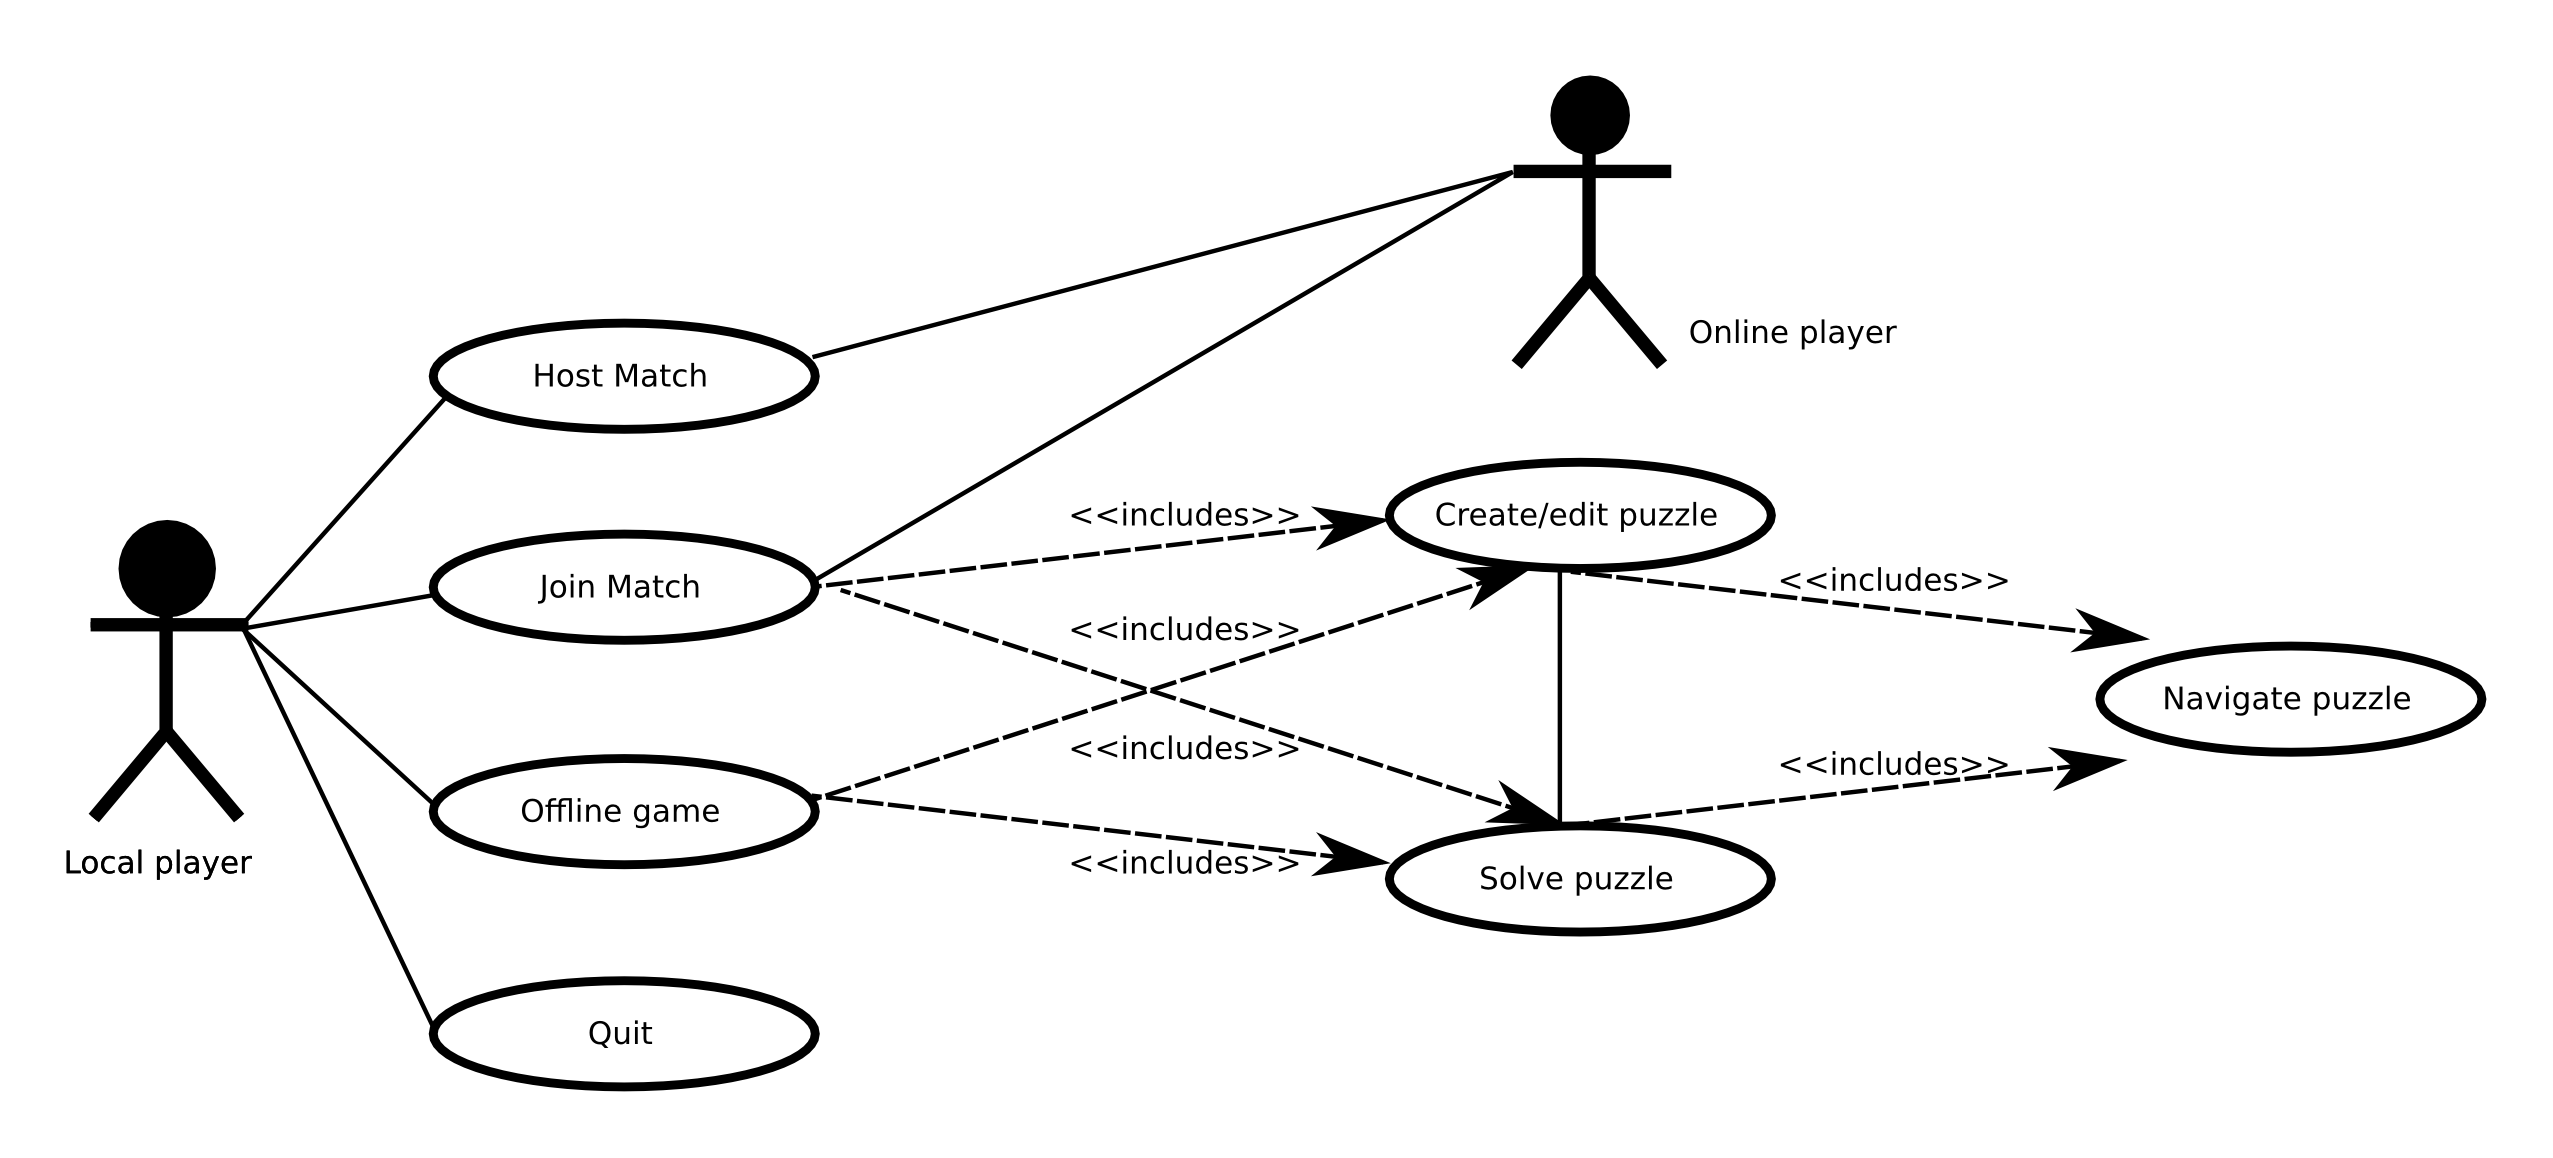
\includegraphics[width=6in]{use_cases.png}
        \caption{Use Case Diagram}
    \end{figure}

\subsection{Actor Descriptions}
    \begin{description}
        \item[Local player] is the local user and has full
            access to the mouse and keyboard or touchscreen interface.
        \item[Online player] is a non-local player. There is two-way
            communication between this type of player and the local player.
            There may be 0 or more online players.
        \item[The Host] has special powers, may disconnect other players and
            block players from selecting different puzzles. This player could
            be Local or Online.
    \end{description}

\subsection{Use-case Descriptions}
\begin{mdframed}
    \subsubsection{Host match}
    \begin{description}
        \item[Entry conditions] Internet connection.
        \item[Exit conditions] Will return to game menu. All players
            disconnected or all puzzles have been solved.
        \item[Participating Actors] Online player and local player.
        \item[Flow of events]:
            \begin{enumerate}
                \item The user presses the appropriate menu button.
                \item User creates a game, selects number of players and game
                    type
                \item User shares (friendly looking) match ID with other
                    players. These players may connect to the match
                \item Puzzle Selector appears.
                \item The user may configure the game with this screen.
                    This
                    entails choosing a puzzle and a game mode (edit or solve).
                    Other players can be prevented from making such
                    modifications.
                \item This Puzzle Selector will create a Puzzle Scene
                \item The scene will change from the main menu to the Puzzle
                    Scene.
                \item Additional view-ports will be added to the game screen.
                These show the progress of online players in an interface
                similar to the local player's puzzle.

            \end{enumerate}
    \end{description}
\end{mdframed}

\begin{mdframed}
    \subsubsection{Join match}
    \begin{description}
        \item[Entry conditions] Internet connection. The menu must be present.
        \item[Exit conditions] Will return to game menu. All players
            disconnected or all puzzled have been solved.
        \item[Participating Actors] Online player and local player.
        \item[Flow of events]:
            \begin{enumerate}
                \item The user presses the appropriate menu button.
                \item Puzzle Selector appears.
                \item The user may configure the game with this screen, if
                    the game host allows it. This would
                    entail choosing a puzzle and a game mode (edit or solve).
                \item This Puzzle Selector will create a Puzzle Scene
                \item The scene will change from the main menu to the Puzzle
                    Scene.
                \item Additional view-ports will be added to the game screen.
                These show the progress of online players in an interface
                similar to the local player's puzzle.
            \end{enumerate}
    \end{description}
\end{mdframed}


\begin{mdframed}
    \subsubsection{Offline game}
    \begin{description}
        \item[Entry conditions] Menu must be present.
        \item[Exit conditions] Will return to game menu. Puzzle has been
            solved.
        \item[Participating Actors] Local player.
        \item[Flow of events]:
            \begin{enumerate}
                \item User selects the appropriate menu button.
                \item Puzzle Selector appears.
                \item The user may configure the game with this screen. This
                    entails choosing a puzzle and a game mode (edit or solve).
                \item This Puzzle Selector will create a Puzzle Scene
                \item The scene will change from the main menu to the Puzzle
                    Scene.
            \end{enumerate}
    \end{description}
\end{mdframed}


\begin{mdframed}
    This use case includes the Host Match, Join Match and Offline Game
    use cases.
    \subsubsection{Edit puzzle}
    \begin{description}
        \item[Entry conditions] A Puzzle Scene must be loaded and edit mode
            must be activated.
        \item[Exit conditions] Will return to game menu. The puzzle may be
            saved to the disk.
        \item[Participating Actors] Online player or local player.
        \item[Flow of events]:
            \begin{enumerate}
                \item The user navigates the puzzle
                \item If a position on the grid is selected, the Block Modifier
                    is presented. This position may be empty or it may
                    contain a block.
                \item The user may change properties of the block using this
                    screen.
                \item Blocks may be added or removed using this same screen.
            \end{enumerate}
            Puzzle preview:
            \begin{enumerate}
                \item User may press the preview button
                \item The user will try the puzzle in Solve Puzzle mode until
                    that mode's exit conditions are met.
                    A special banner will graphically indicate preview mode.
                \item The solving scene will have a special button for
                    returning to the editing scene
            \end{enumerate}
    \end{description}
\end{mdframed}


\begin{mdframed}
    This use case includes the Host Match, Join Match and Offline Game
    use cases.
    \subsubsection{Solve puzzle}
    \begin{description}
        \item[Entry conditions] A Puzzle Scene must be loaded and solve mode
            must be activated.
        \item[Exit conditions] Will return to game menu or puzzle editor.
            If the game is over, an overview of results will be shown and the
            steps taken to solve the puzzle may be saved to the disk.
        \item[Participating Actors] Online player or local player.
        \item[Flow of events]:
            \begin{enumerate}
                \item The user navigates the puzzle
                \item If a block is selected, the block runs any associated
                    Block Action.
                \item These Block Actions may modify the block's properties or
                    request the addition or removal of blocks, including the
                    selected block, from the Grid Manager.
                \item This sequence is repeated until the winning block is
                    found, the user quits, or a losing condition is met.
                \item User's actions may be mirrored on an online player's
                    screen, likewise, separate Puzzle Scenes  may be updated
                    with any moves made by other players.
            \end{enumerate}
    \end{description}
\end{mdframed}


\begin{mdframed}
    \subsubsection{Navigate puzzle}
    This use case includes the Solve puzzle and Edit puzzle use cases.
    \begin{description}
        \item[Entry conditions] Puzzle scene loaded and permission to move.
            Input devices must be functional.
        \item[Exit conditions] The game must offer continuous feedback.
            If the entry conditions are met, any further input must be
            acted on as soon as possible.
        \item[Participating Actors] Online player and local player.
        \item[Flow of events]:
        	\\
            Camera motion:
            \begin{enumerate}
                \item User drags with a mouse or touchscreen
                \item The camera changes position
            \end{enumerate}

            Block selection:
            \begin{enumerate}
                \item User clicks with mouse or taps on touchscreen
                \item The 3D coordinates are translated into a position on
                    a game ``board.''
                \item The Grid Manager is notified of input and the grid
                    position.
                \item If a block is present there, it is selected and activated.
                    Exact actions depend on the game mode.
                \item If a block is not present, the space is selected. This
                    is only useful in edit mode.
                \item The user may end the game at any point through the pause
                    menu.
            \end{enumerate}

    \end{description}
\end{mdframed}


\begin{mdframed}
    \subsubsection{Quit}
    \begin{description}
        \item[Entry conditions] Game must be running. This action is
            asynchronous and may activate at any point.
        \item[Exit conditions] Game, be gone!
        \item[Participating Actors] Local player.
        \item[Flow of events]:
            \begin{enumerate}
                \item User presses the quit button on a menu
                \item or User presses appropriate sequence of keys, such as
                    the escape key or the alt and F4 combo.
                \item Some data may be saved, such as the puzzle being currently
                edited.
                \item The program shuts down gracefully.
            \end{enumerate}
    \end{description}
\end{mdframed}



\section{Architectural Design}
% HR
\subsection{Subsystem Architecture}
% SM
\begin{figure}[H]
    \centering
    
\includegraphics[width=0.8\linewidth]{subsys_arch.png}
    \caption{Layered Subsystem Architecture UML Diagram.}
\end{figure}
The two primary subsystems of Anttris are the puzzle system and the online system.

The puzzle-solving system is composed generically over a puzzle viewer and attached event
handling that allows interaction with the puzzle. Both offline games and online ones use
the puzzle viewer, as does the unique puzzle-editing mode. The puzzle viewer is used by
all three unique modes, and works with our 3D model interaction system to provide
interactivity. This system is built on the Godot 3d Engine, which uses OpenGL.

The online system breaks down immediately into host mode or remote client mode. The host
mode interfaces with the application-generic session-host system, which works in conjunction
with the session lobby to facilitate remote clients to connect and play against the host.
Remote clients also work closely with the session lobby to find hosts to play against. Both
the session lobby and the session-host system work with the Godot Online Subsystem to provide
connectivity. The Godot Online Subsystem is built over tcp-udp/ip.

\subsection{Deployment Model}
% HR
\section{Use Case Realization Design}
% HR, I did Use Cases last time, I can work on all of this
\section{Subsystem Design} % CA
Anttris is broken down into the following four subsytems: GUI, Networking, File Manager and Game.
\subsection{Anttris GUI} % CA
    \begin{figure}[H]
        \centering
        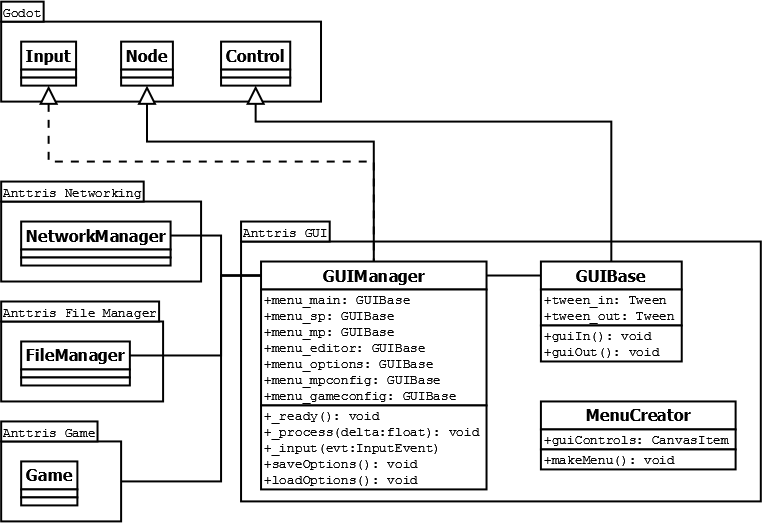
\includegraphics[width=6in]{Anttris_GUIClass.png}
        \caption{Class diagram for the GUI subsystem.}
    \end{figure}
    \begin{figure}[H]
        \centering
        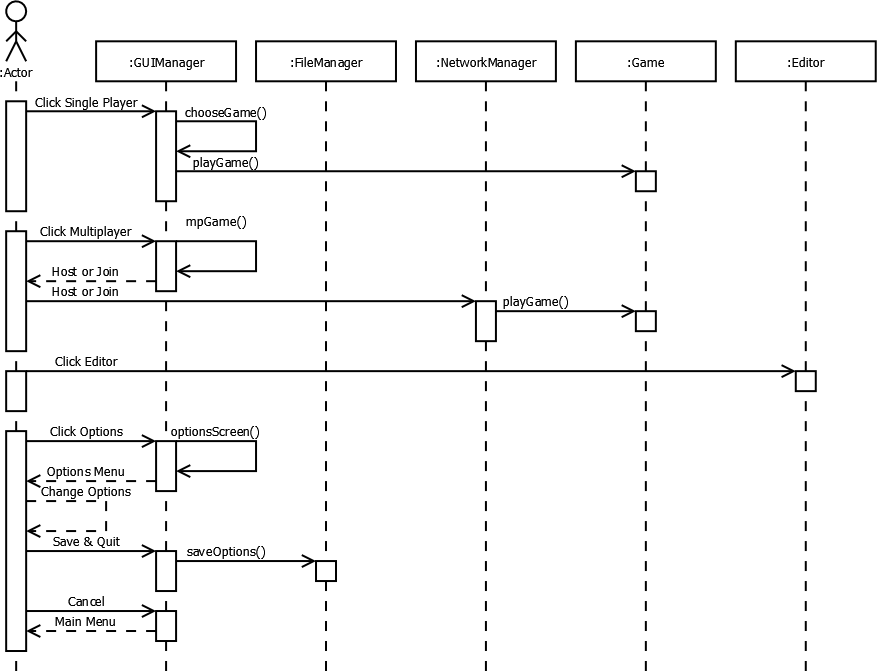
\includegraphics[width=6in]{Anttris_GUISequence.png}
        \caption{Sequence diagram for the GUI subsystem.}
    \end{figure}

This subsystem manages all of the graphical user interfaces that make up the menus. Menus all inherit GUIBase to provide smooth and consistent fade in and slide out animations. The MenuCreator just takes all of the buttons in a menu and orders them nicely for consistency. The menus themselves will be object instances of GUIBase.

\subsection{Anttris Network Manager} % CA
    \begin{figure}[H]
        \centering
        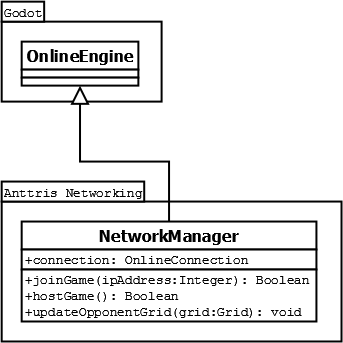
\includegraphics[width=2.7in]{Anttris_NetworkingClass.png}
        \caption{Class diagram for the networking subsystem.}
    \end{figure}

This subsystem will provide a central interface for networking. All games that are joined or hosted for competitive play will go through this subsystem. It updates the connection periodically and updates the opponents grid on the screen when they make new moves. This subsystem has no sequence diagram as it is self contained and is only used by outside subsystems. See the sequence diagrams for the GUI and game subsystems.

\subsection{Anttris File Manager} % CA
    \begin{figure}[H]
        \centering
        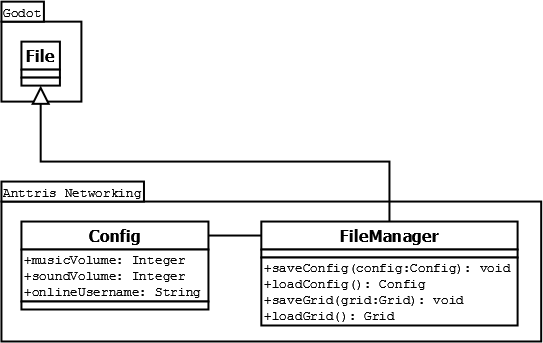
\includegraphics[width=4.27in]{Anttris_FileClass.png}
        \caption{Class diagram for the networking subsystem.}
    \end{figure}

This subsystem will provide a central interface for file management. Options will be loaded and saved from here as well as any puzzles created in the editor.
\section{Human Interfaces} % CA / SM
    \begin{figure}[H]
        \centering
        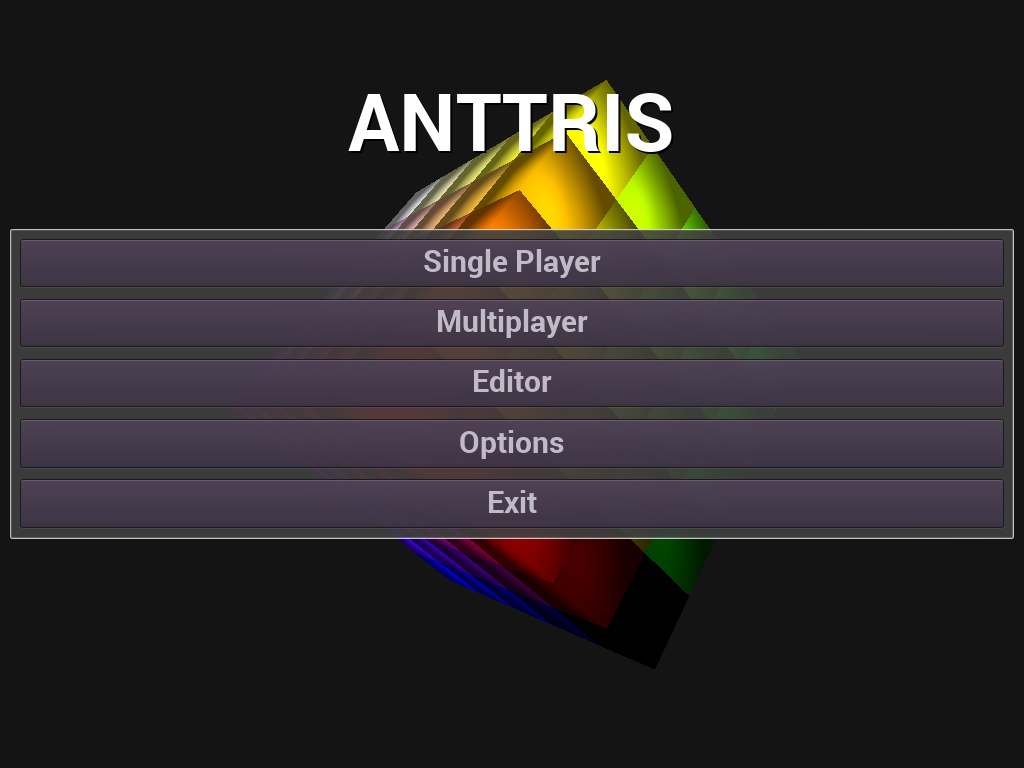
\includegraphics[width=4.5in]{Anttris_MainMenu.png}
        \caption{Main menu design.}
    \end{figure}
    \begin{figure}[H]
        \centering
        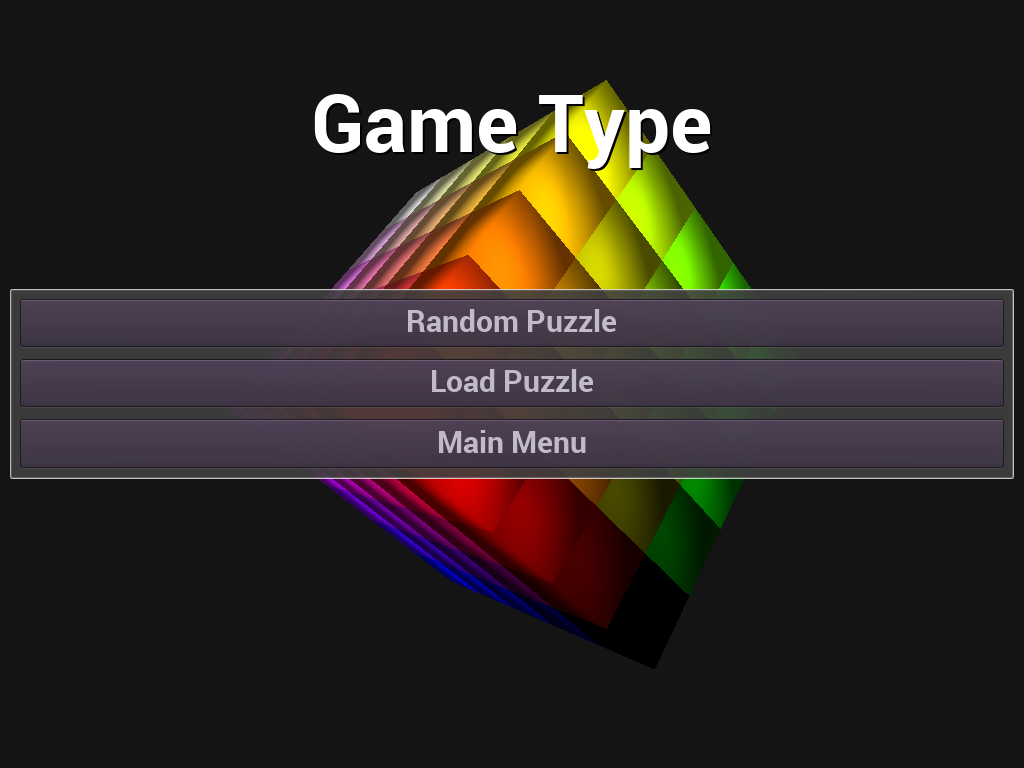
\includegraphics[width=4.5in]{Anttris_GTMenu.png}
        \caption{Game type menu design.}
    \end{figure}
    \begin{figure}[H]
        \centering
        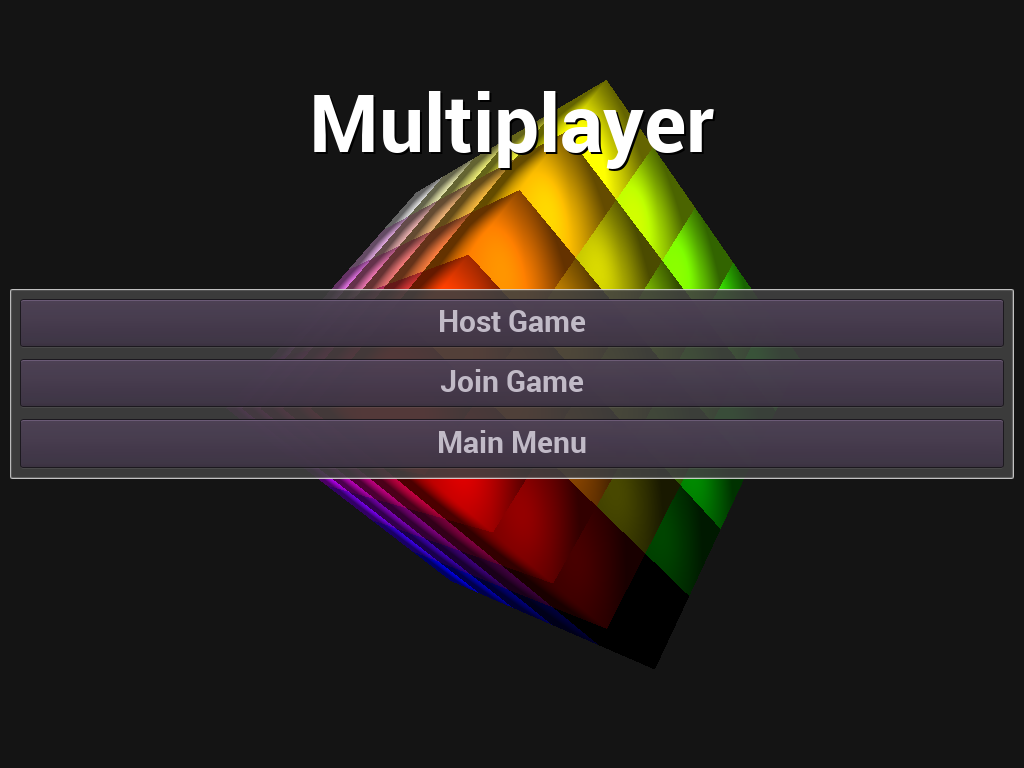
\includegraphics[width=4.5in]{Anttris_MPMenu.png}
        \caption{Multiplayer menu design.}
    \end{figure}
    \begin{figure}[H]
        \centering
        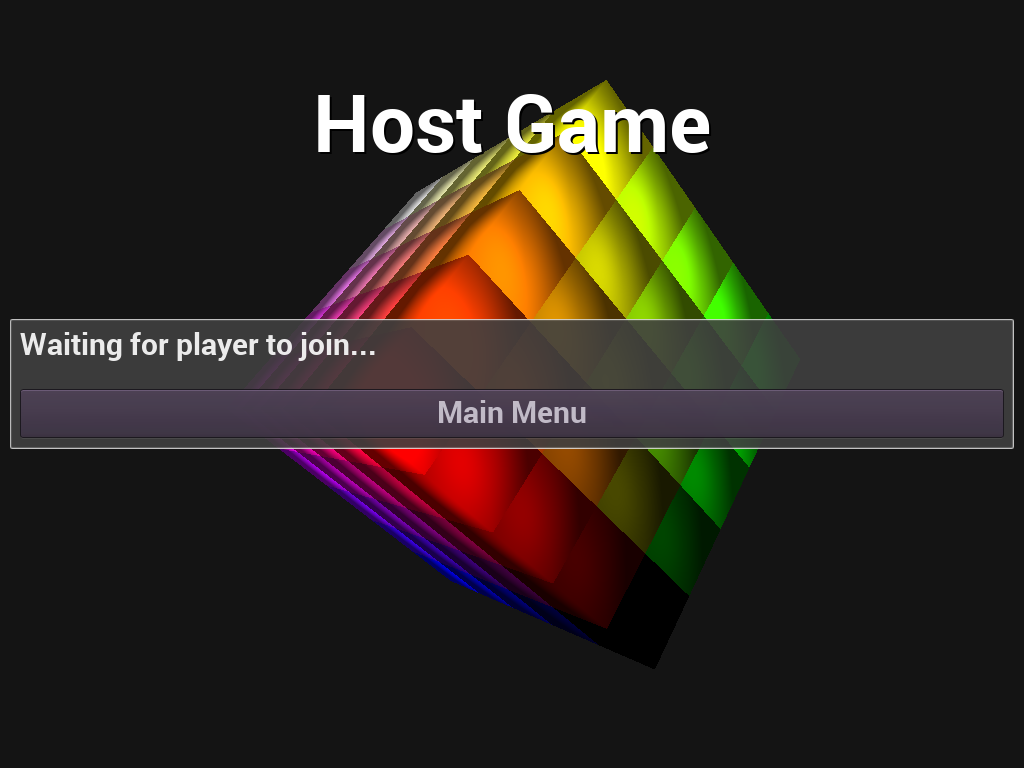
\includegraphics[width=4.5in]{Anttris_HGMenu.png}
        \caption{Host game menu design.}
    \end{figure}
    \begin{figure}[H]
        \centering
        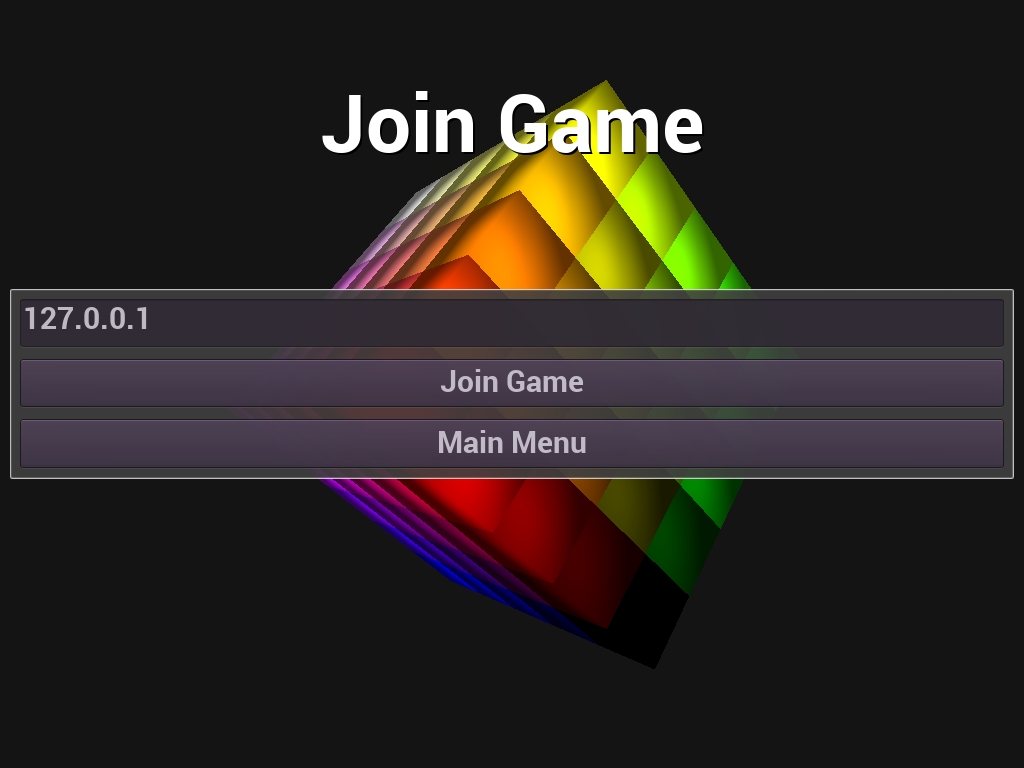
\includegraphics[width=4.5in]{Anttris_JGMenu.png}
        \caption{Join game menu design.}
    \end{figure}
    \begin{figure}[H]
        \centering
        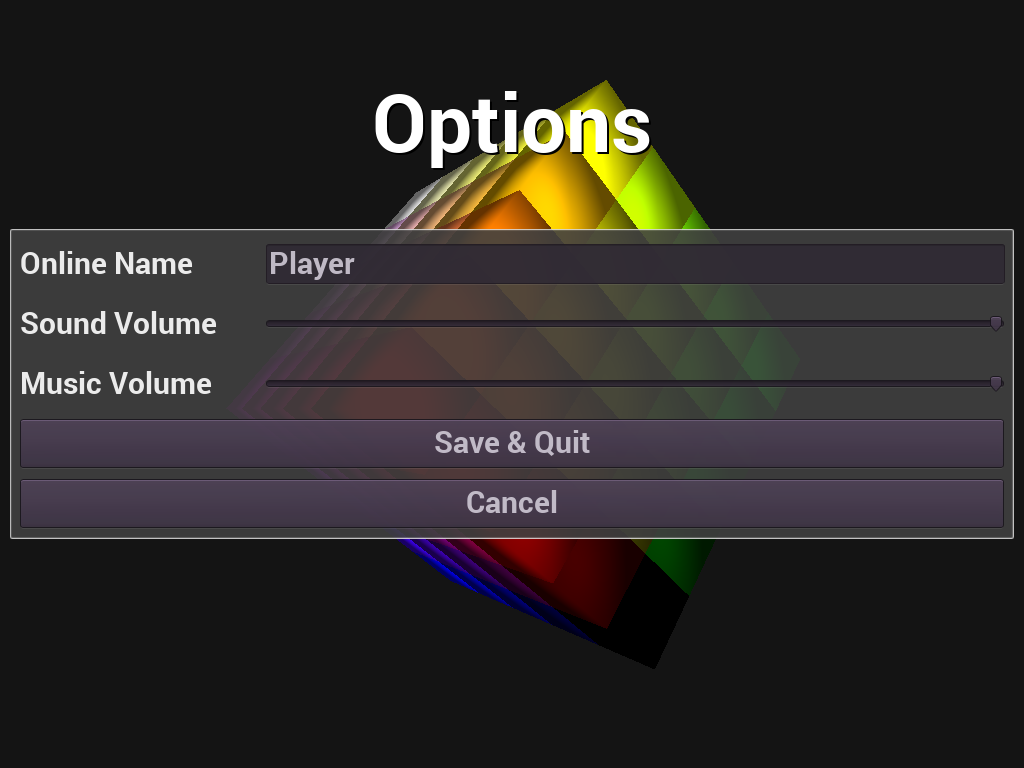
\includegraphics[width=4.5in]{Anttris_OptionsMenu.png}
        \caption{Options menu design.}
    \end{figure}
\section{System/Data Dependencies \& Requirements}
% ST, BC
\section{Testing Plan}
8. Testing Plan

In order to test that the game is working properly we will be using Black Box and White Box testing methods. Using these methods we can test the game from the outside-in by making sure that the functionality of the interface preforms the correct actions then working our way to the coding level. This approach will prevent more errors and bugs in the early stages of testing, since we will not be working with the code directly at the start. Any errors and bugs we encounter will be documented and recorded for future reference.

For the first part of the testing plan, we will be testing the game on multiple physical computers to make sure the interface of the game preforms correctly. Testing the game on multiple machines will allow for a diverse testing experience, and will confirm whether or not our game can work on multiple systems. Once we know the game can run on each of the tested machines, we will begin testing the interface of the game.
The interface of the game is what the user will be interacting with, so we want to make sure that the interactions of each function work correctly and display the correct information to the user. To test the interface of the game we will:

\begin{enumerate}
\item Test the menu options
\item Test Single-Player Game Mode (Single-player, New Game, Continue Game)
\item Test Puzzle Editor/Creator: (Create, Edit, Delete)
\item Solve basic test puzzles (Test Puzzle 1, 2, 3,...)
\item Multiplayer Game Mode
\end{enumerate}

Testing Menu Options:
In order to test the menu options, we will click on each of the options and make sure that the selected menu option displays the next options or pages the user needs to see. For instance, if a user selects “single-player game”, we don't want the game pulling up the information for a multiplayer game.
We will be testing each of the options the user may choose from and if the user can reselect options by returning to the previous options. Since this is the first thing the user will see when playing our game, and is what decides what type of games the user will be playing, we can to make sure they work properly and don't cause the game to close unexpectedly.

Test Single-Player Mode:
Once we know all the menu options work correctly, we will test the Single-Player Game Mode. In Single-player, the user will be able to select whether they wish to start a new game or continue a game they left off on. The New Game option will allow the user to select the puzzle they wish to play and solve that puzzle from the beginning. In order to test this option, we will have a set number of puzzles generated and we will test each puzzle separately on each machine. We want to make sure that the puzzle generates the correct puzzle and generates the same way each time. After testing the new game function, we will test the continue function. This function allows the user to continue from a saved game file and will allow the user to continue solving the puzzle.

Test Puzzle Editor/Creator:
After we have tested the New Game and Continue functions, we will be testing the puzzle editor functions which are accessed in the Single-Player Mode. The puzzle editor is where the user can create new puzzles, edit previously made puzzles, and delete puzzles they may not want anymore. In order to test creating new puzzles, we will be creating basic puzzles, seeing if we are allowed to place blocks on the grid correctly, and if the game will catch any errors when saving the puzzle. When creating basic puzzles we will be using the in game tools to create and remove blocks on the grid. We will need to test that we can place each type of block, and be able to remove each type of block when placed on the grid. Testing the edit puzzle option is similar to the create new puzzle option, except when editing a puzzle we need to make sure that the puzzle the user wishes to edit appears correctly so the user can make the proper changes.

Solving Puzzles:
After we have tested the Puzzle Editor, we will attempt to solve puzzles. Using per-constructed, basic puzzles, we will solve each of the puzzles and confirm that each of the blocks preforms the correct action when clicked, and test if the game records scores correctly and ends when the goal block is reached. Each of the tester puzzles, will consist of each type of block and possible interactions so we can make sure that the game flow is not ruined when blocks preform their actions. Solving Puzzles is the last step in testing the Single-Player mode and is the most important.

Multiplayer Game Mode:
Multiplayer Game Mode will be the last thing we test since it involves the interactions between two computers. We will be testing the Create and Host Match options like we did the menu options and the different game modes similarly to the Single-Player and Multiplayer game modes. The most important thing we need to test for the multiplayer are the interactions between the two players. In order to test the interactions, we need to make sure that two players are able to connect to each other and preform actions in the interface and when solving puzzles with each other.

After testing the interface of the game and making sure each of the game options and modes work correctly, we will review errors and bugs we encountered during the Black Box testing. Upon completion we will need to begin White Box testing and testing that the correct values are being passed in the code.
% ST, BC
\section{Appendices}
% ST
\subsection{Project Status}
% ST
The project is coming along nicely. Thanks to this document, we now have a clearer idea for the design of the subsystems of the game.

We've divided the responsibilities up amongst ourselves roughly as follows: Chris is working with Benji and Skyler on the core game coding (puzzle generation and solving.) Graphics and textures are being worked on by Benji and Chris. Hugo and Skyler are working on the block logic. Testing will be carried out by everyone. Sean is still acting as Scrum master and will be responsible for code quality and documentation. As usual, however, everyone will pitch in where needed.

Spring break wasn't hugely productive...as we expected...but we've spent some time learning the Godot engine and working on an early version of the game.

We are on track to start another sprint this week, which will enable us to hopefully get core functionality working. The plan is to get a core game working. Once that is done, we plan to spend the remaining time in the semester working on advanced features and documentation.

\bibliographystyle{acm}
\bibliography{team5-design-spec}
\end{document}
